% ======================================================= %
%                       Introduction                      %
% ======================================================= %
\section{Background}

    % --------------------------------------------------- %
    %                  Motivation:Goals                   %
    % --------------------------------------------------- %
    \subsection*{Motivation}
    \begin{frame}{Goals}
        Simulate a simple closed-loop with naturally circulating water in both single and two-phase regimes using
        \begin{Itemize}
            \item{Non-ideal equation of state for water}
            \item{Simple but accurate models for frictional pressure losses}
            \item{Modern, nonlinear solver with complete residual convergence}
            \item{Rigorous discretization that allows for exact integration of conservation equations over physical domain}
        \end{Itemize}
        
        And ultimately determine the linear stability of the system under consideration.
    \end{frame}
    
    % --------------------------------------------------- %
    %             Motivation:Leading Questions            %
    % --------------------------------------------------- %
 \begin{frame}{Stability}
        \only<1>{
        What is stability?
            \begin{Itemize}
                \item{Often used term}
                \item{Used with many definitions (both implicit and explicit)}
            \end{Itemize}
        }
        
        \only<2>{
        One definition:
            \begin{beamercolorbox}[sep=0.4em,rounded=true]{titlelike}
                Transient (possibly oscillatory) thermal hydraulic phenomenon stemming from 
                nonlinear-geometric-multiphase feedback that could lead to system excursions 
                causing dangerous mechanical or thermal damage and possibly human harm.
            \end{beamercolorbox}
        }
        
        \only<3-4>{
        Another definition:
            \begin{beamercolorbox}[sep=0.4em,rounded=true]{titlelike}
                A system of the form
                \begin{equation}
                    \partial_{t} q = f(t,q)
                \end{equation}
                is stable if $q \in [q_{\text{low}},q_{\text{hi}}]$ for all time.
            \end{beamercolorbox}
        }
        
        \only<4>{
            Definition for here:
            \begin{beamercolorbox}[sep=0.4em,rounded=true]{titlelike}
                A system of the form
                \begin{equation}
                    \partial_{t} q = A q
                \end{equation}
                is stable if all eigenvalues of $A$ are less than or equal to zero.
            \end{beamercolorbox}
        }
        \only<5>{Applications?
                \begin{Itemize}
                    \item<2->{Thermosiphon}
                    \item<2->{Power cycle loops}
                    \item<2->{And... }
                 \end{Itemize}
        }
    \end{frame}




    % --------------------------------------------------- %
    %                 RCCS:Overview                       %
    % --------------------------------------------------- %
    \subsection*{RCCS}
    \begin{frame}{Reactor Cavity Cooling System}
        \begin{columns}
            \begin{column}[T]{0.45\textwidth}
                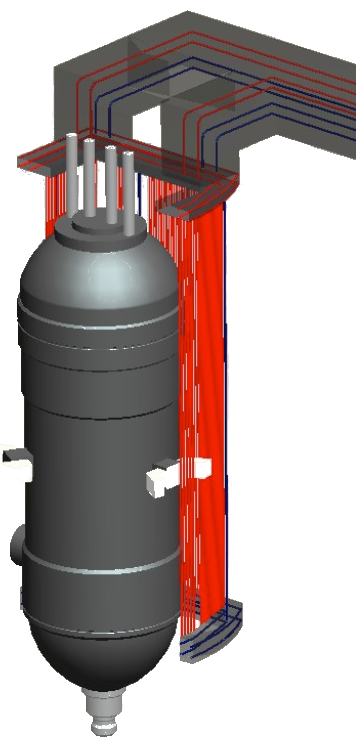
\includegraphics[height=2.5in]{RCCSMockup}
            \end{column}
            \begin{column}[T]{0.45\textwidth}
                \textbf{Purpose:}\hfill\\
                Naturally-driven cooling of reactor under accident conditions
                
                \vspace*{2em}
                \textbf{Accident conditions:}\hfill\\
                Loss of onsite, offsite power (station blackout)
            \end{column}
        \end{columns}
    \end{frame}
    

    \begin{frame}{Reactor Cavity Cooling System: Big picture}
    \begin{columns}<1>
        \begin{column}[T]{0.45\textwidth}
            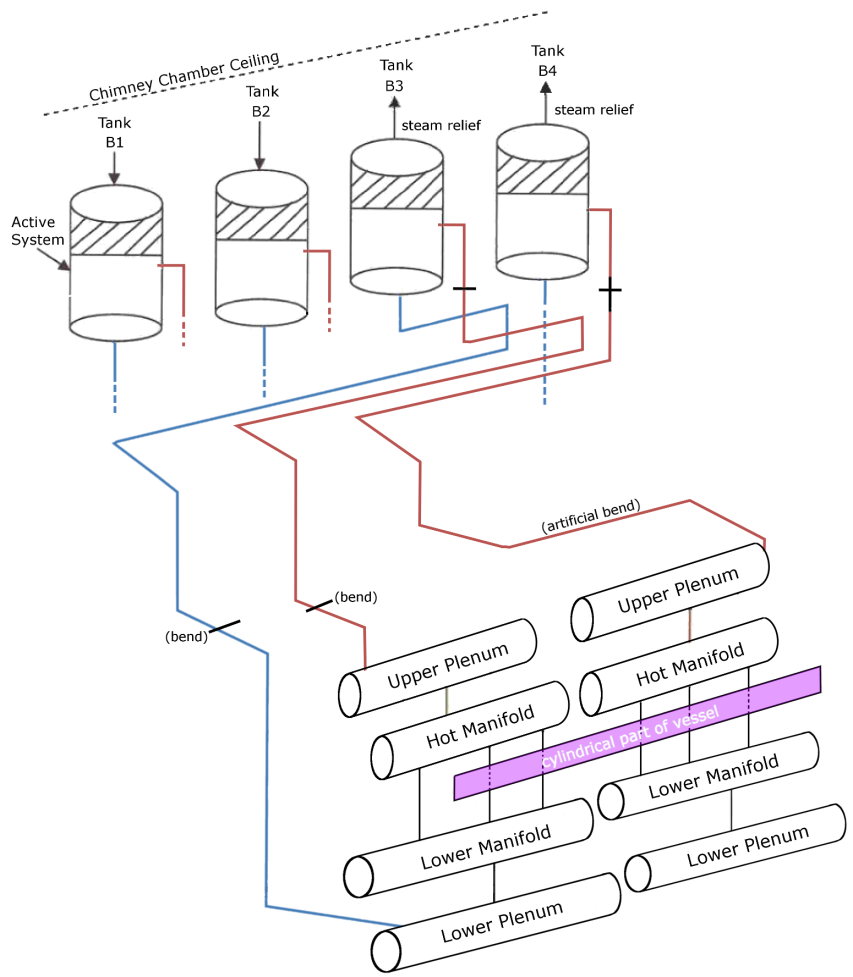
\includegraphics[height=2.5in]{RCCSTotalSystem}
        \end{column}
         \begin{column}[T]{0.45\textwidth}
            \textbf{Selected specifications:}\\[0.2em]
            \begin{Itemize}
                \item{Trains: 2}
                \item{Lines/Tanks: 8}
                \item{Elevation change: 35 meters}
                \item{Path length: 200 meters}
                \item{Heated length: 20 meters}
                \item{Risers: 200+}
                \item{Heat transfer:}
                \begin{Itemize}
                    \item{Radiation: 80\%}
                    \item{Convection: 20\%}
                \end{Itemize}
            \end{Itemize}
        \end{column}
    \end{columns}
\end{frame}


    % --------------------------------------------------- %
    %                 RCCS:Experiment                     %
    % --------------------------------------------------- %
    \begin{frame}[c]{RCCS Experiment}
        \begin{columns}[c]
            \begin{column}{0.35\textwidth}
                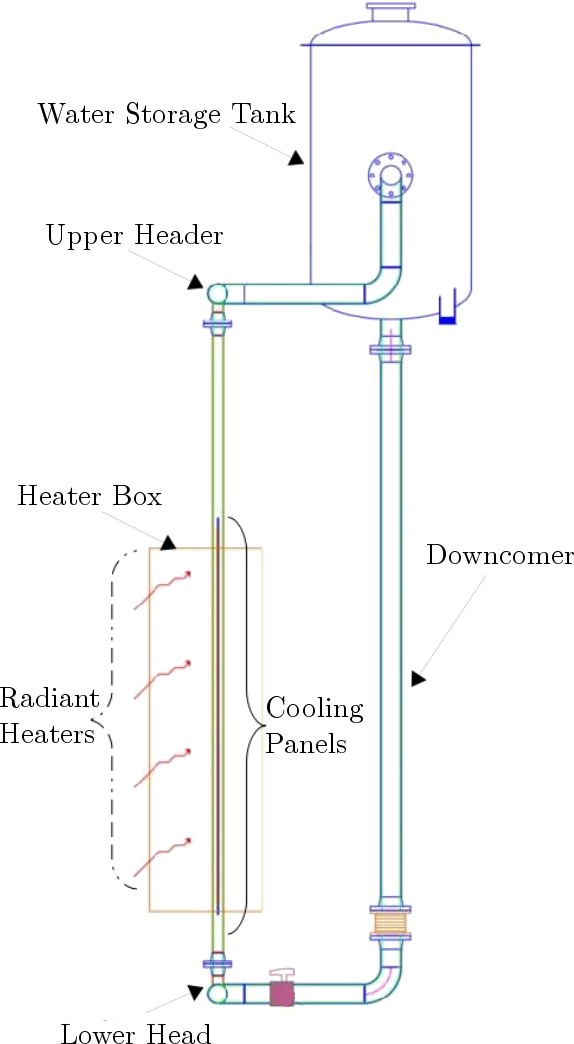
\includegraphics[height=2.5in]{RCCSExperimentOverview}
            \end{column}
            \begin{column}{0.60\textwidth}
                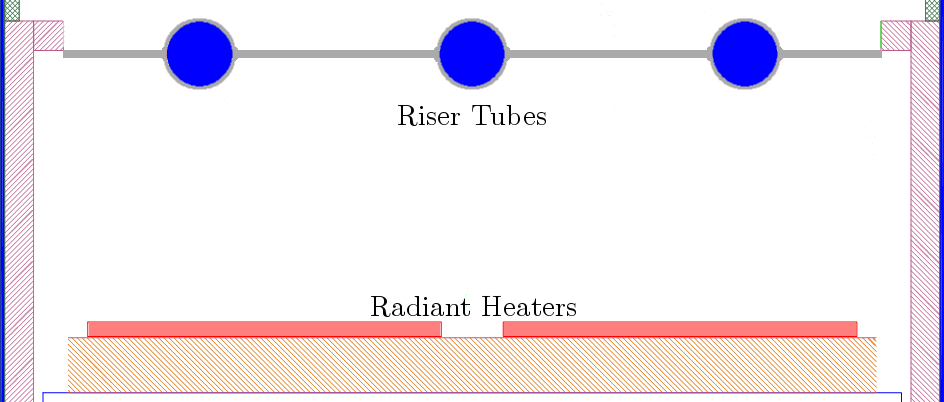
\includegraphics[width=2.5in,angle=0]{RCCSExperimentHeatBox}
            \end{column}
        \end{columns}
    \end{frame}
    
    
    
    % --------------------------------------------------- %
    %                 RCCS:Mass Flow rate                 %
    % --------------------------------------------------- %
    \begin{frame}[c]{Experimental data: flow oscillations during boiling}
        \begin{center}
            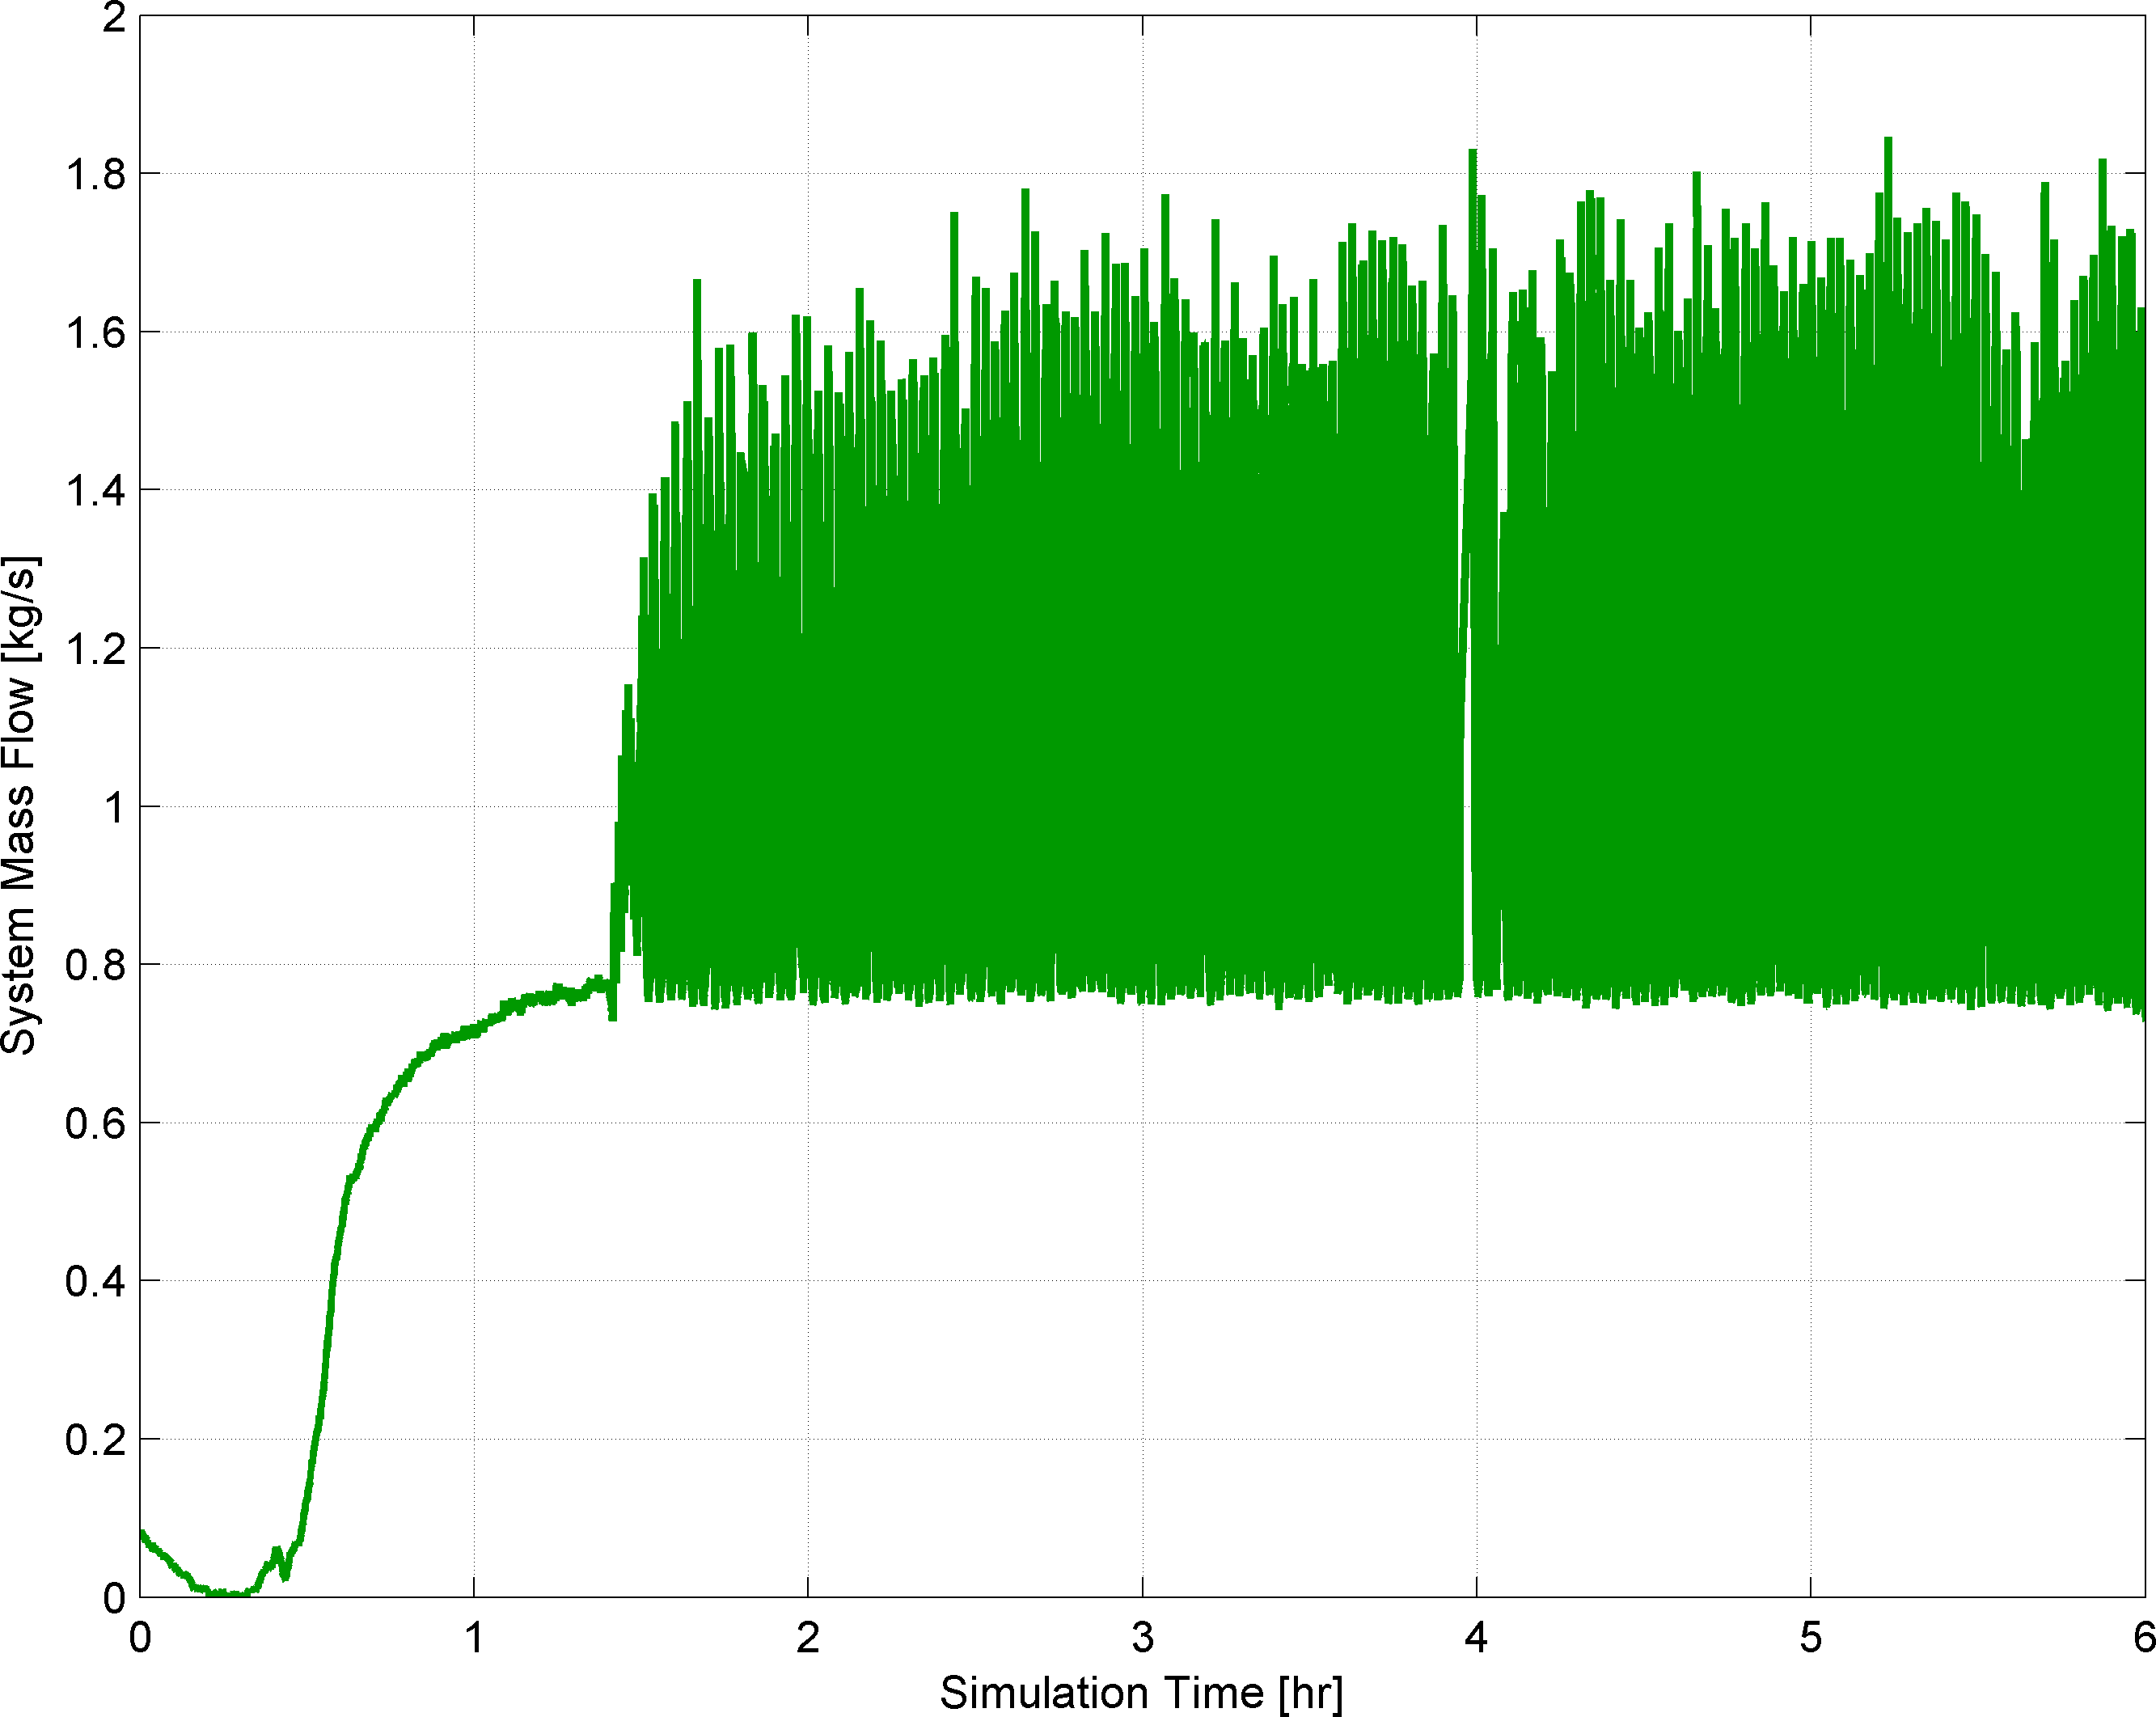
\includegraphics[height=2.5in]{ExperimentMassFlow}
        \end{center}
    \end{frame}



    % --------------------------------------------------- %
    %                     Literature                      %
    % --------------------------------------------------- %
    \subsection*{Literature}
    \begin{frame}{Been done before?}
        Two-phase, natural circulation stability in the literature exists (see thesis).
        \vspace{1em}
        But...
        \begin{Itemize}
            \item{Analytical work limited to simple equations-of-state}
            \item{Large volumes with piece-wise properties (non-dimensional numbers abound)}
            \item{System code usage hindered by simple discretization scheme and confounded by complicated models}
        \end{Itemize}
    \end{frame}
